\section{Aims and Objectives}
The aim of this project is to develop an Internet of Things (IoT) system to regularly monitor the health of the Griffith footbridge through three dimensional vibration analysis. The high level system of this project comprises of three sensor nodes placed across the length of the footbridge that transmit packets over the LoRaWAN protocol. These packets are received by a gateway placed at the end of the bridge and are uploaded to The Things Network (TNN) cloud for data processing. Arduino MKR 1300 and 1310 boards will be used as the carrier boards for these sensor nodes. Figure \ref{fig:HL-HW-Diagram} shows the high level hardware diagram for this IoT system.  

\begin{figure}[h!]
\center
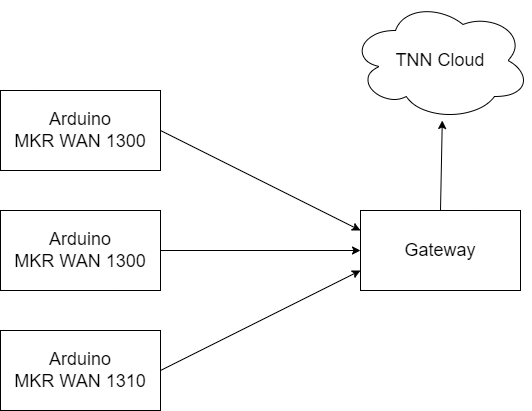
\includegraphics[scale=0.35]{Images/HW-Diagram.png}
\caption{High Level Hardware Diagram}
\label{fig:HL-HW-Diagram}
\end{figure}

Each sensor node will include an accelerometer to detect, log and transmit movement in three dimensions (x, y and z axis). This data is sent to the on-board processor of the Arduino carrier board where it is logged. The average movement on each axis as averaged and sent via data packet over LoRaWAN via a dipole antenna every hour. The carrier board itself is powered with a simple solar panel / battery setup. The pro gateway is listening for packets on the LoRa network via a mono-pole antenna. These packets are then sent to the on board Raspberry Pi 3 model B+ processor. The processor transmits these packets to the TNN cloud. This more detailed system can be seen in figure \ref{fig:HL-HW-Diagram-Detailed}.

\begin{figure}[h!]
\center
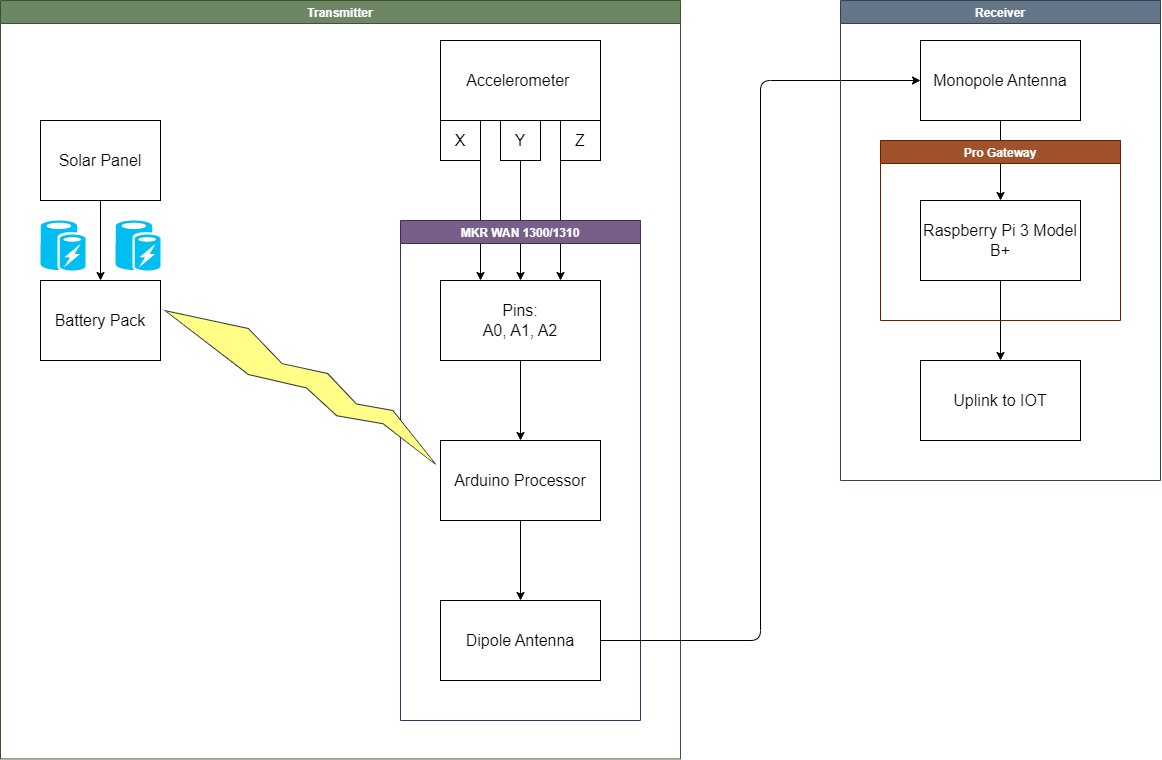
\includegraphics[scale=0.35]{Images/HW-Diagram-Detailed.png}
\caption{Detailed High Level Hardware Diagram}
\label{fig:HL-HW-Diagram-Detailed}
\end{figure}

\begin{figure}[h!]
\center
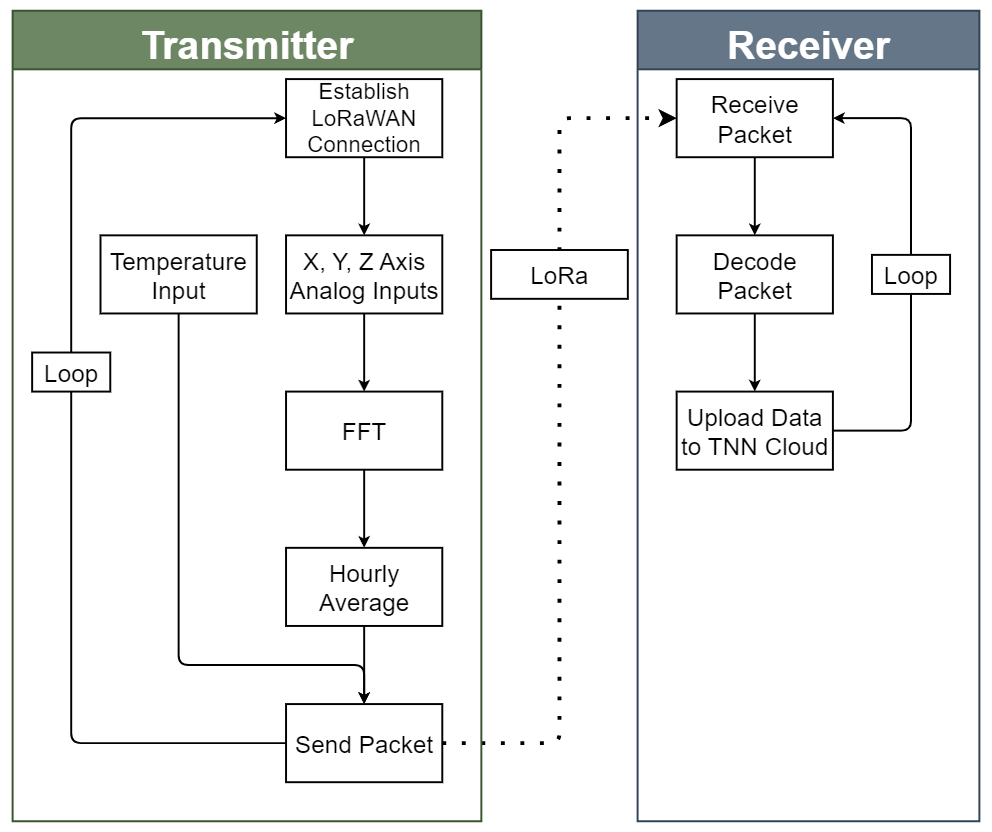
\includegraphics[scale=0.35]{Images/SW-Diagram.png}
\caption{High Level Software Diagram}
\label{fig:HL-SW-Diagram}
\end{figure}

Figure \ref{fig:HL-SW-Diagram} displays the higher level software diagram for the transceiver and receiver.  One of the major aims of the project will be to further explore this software design which is heavily dependent on the functional requirements of the system. The functional requirements of the system will  dictate the packet size and transmission frequency. Additionally, different types of windowing techniques for the Fast Fourier Transform will be explored to remove noise from accelerometer analog inputs. 

\subsection{Funtional and Non-Functional Requirements}
The funcional and non-functional requirements in table \ref{tab:FRandNFR} form the basis of the measurable objectives that need to be met. Meeting these defined objectives will satisfy the aims of this project. 

\begin{longtable}{ | p{3.5cm} | p{1.25cm}| p{4.5cm} | p{4.5cm} | } 
\hline
\textbf{Requirement}& \textbf{Status}& \textbf{Description}& \textbf{Verification Method} \\
\hline
[FR-1] The transmitter and receiver shall communicate at a frequency of 925MHz& Draft& The frequency band for LoRaWAN in Australia is 915-930MHz so the IoT network must operate within this range& This requirement can be verified through integration testing and observing packet transmition via test application \\
\hline
[FR-2] The gateway shall receive packets from a distance of up to approximately 600m& Draft& LoRa communication is advertised to operate within multiple kilometers but the system will only need to operate approximately up to 600m& The range of the system can be verified through integration testing by noting the distance at which packet loss occurs \\
\hlinett
[FR-3] The receiver shall receive packets and distinguish between at least three sensor nodes& Draft& The IoT system requires at least three sensor nodes to be placed along the bridge. It is therefore required that each transmitted packet contains an identifier& The identification of transmitted packets can be identified trough integration testing and observing packet transmission via a test application \\ 
\hline
[FR-4] The sensor nodes shall be powered by solar energy such that the nodes can transmit 24/7& Draft& The nodes need to transmit packets every hour 24/7 and hence require a solar battery system capable of supporting always-on low powered devices& The current draw from the sensor nodes can be measured and the appropriate power supply can be calculated. Otherwise field testing will be required to examine how long the sensor nodes can operate for \\
\hline
[FR-5] 	Each sensor node shall include an accelerometer to record analog input on the x, y and z axis& Draft& The accelerometers will measure the bridge's vibration. This data will be converted into digital data using Fourier transform techniques and encoded into packets& The accelerometers will be tested in the mechanical engineering lab with a vibrating beam setup \\
\hline
[NFR-1] 	The sensor nodes shall be resistant to overheating and rain& Draft& The sensor nodes will be exposed on the bridge and will therefore have to survive hot temperatures and rainfall& The enclosure will be designed with weather proofing in mind and will undergo laboratory environmental testing \\
\hline
[NFR-2] 	The sensor nodes shall contain temperature and humidity sensors and transmit this data& Draft& 	Temperature and humidity data will be useful to spot any discrepancies in the data due to external environment and will be useful to field test the thermal resistance of the device enclosure. The data from these sensors will be included in the transmitted packets along with the vibration data& The operational capabilities of these sensors can be examined in a lab. The functional capabilities of these sensors will need to be tested in the field \\
\hline
\caption{Functional and Non-Functional Requirements}
\label{tab:FRandNFR}
\end{longtable}



